\label{experiments}

The following hyperparameters were constant during all of the experiments:
\begin{table}[H]
\centering
\begin{tabular}{|l|c|}
\hline
\textbf{Hyperparameter} & \textbf{Value} \\ \hline
Train Split & 0.8 \\ \hline
Validation/Test Split & 0.5 \\ \hline
Model Type & \ac{FNN} \\ \hline
Optimizer & Adam \\ \hline
\end{tabular}
\caption{Hyperparameters: Common}
\end{table}

\section{Subcortical Segmentation}

This simple problem did not need a lot of tuning, as it was working very well almost from the start. The following set of hyperparameters were constant during these experiments:
\begin{table}[H]
\centering
\begin{tabular}{|l|c|}
\hline
\textbf{Hyperparameter} & \textbf{Value} \\ \hline
Control/Huntington Datapoints & Control Only \\ \hline
Left/Right Hemisphere Datapoints & Both \\ \hline
Space & Native \\ \hline
Image & T1 \\ \hline
Scaling/Normalization & Normalized Voxel Based Features \\ \hline
Hidden Layers & 1024 \rightarrow 512 \rightarrow 256 \rightarrow 128 \\ \hline
Loss & Categorical Crossentropy \\ \hline
Activation & Sigmoid (softmax for the output layer) \\ \hline
Learning Rate & 0.001 \\ \hline
Batch Size & 10000 \\ \hline
Early Stopping Patience & 7 \\ \hline
\end{tabular}
\caption{Hyperparameters: Subcortical}
\label{tab:subhyp}
\end{table}
The reasoning behind the initial choices of these parameters are straight forward. The T1 image and native space were chosen, because those are the simplest to acquire in practice. Thus if the model is doing great on those, there is no need for more complicated inputs. Including both hemispheres would hopefully result in a model which can generalize better. Only using control datapoints should translate into less variance between the general characteristics of the datapoints, as it does not contain patients with neurodegeneration. The number and sizes of the hidden layers were choosen based on the potential size of the input layer, which should range from $92$ (single set of voxel based features) up to $\sim1000-2000$ including many different kernel sizes and non-voxel based features as well. Categorical crossentropy loss function and the output layer's softmax activation function are standard practices for a classification problem. The Sigmoid activation function should work fine without having to deal with exploding gradients and dieing relu problems. Learning rate is the default learning rate of the Adam optimizer in TensorFlow. And a batch size of $10,000$ seems appropriate for a train split size of $1,000,000$ datapoints. And the early stopping patience of 7 epochs should also be good enough to prevent overfitting and stop the training in time, but it will be evaluated based on the learning curves and the accuracy of the model.\par
The used metric for evaluating model performance on the Train/Validation/Test splits is Accuracy. The 'k' and 'b' notations stand for kernel and bin, where k5 means a kernel width of 5mm, b25 means an absolute bin size of 25, and b10r means relative binning with 10 bins. And in the case of multiple kernel sizes denoted by a dash, it naturally only means odd kernel sizes. Tuning the rest of the hyperparameters were done in the following experiments:

\begin{longtable}[H]{|r|p{9cm}|l|l|l|r|}
\hline
 & \textbf{Experiment} & \textbf{Train} & \textbf{Val} & \textbf{Test} & \textbf{Input Layer} \\ \hline
1. & \textbf{Voxel Features k5\_b25} & $68.9$ & $69.1$ & $72.4$ & $92$  \\ \hline
2. & \emph{Voxel Features k5\_b25} \newline \textbf{Non-Voxel Features of Target Regions b25} & $73.2$ & $68.9$ & $72.5$ & $1576$ \\ \hline
3. & \emph{Voxel Features k5\_b25} \newline \textbf{Non-Voxel Features of ROI b25} & $75$ & $74.3$ & $78.5$ & $304$ \\ \hline
4. & \emph{Voxel Features k5\_b25 \newline Non-Voxel Features of ROI b25} \newline \textbf{Non-Voxel Features of Brain b25} & $74.5$ & $70.4$ & $70.3$ & $410$ \\ \hline
5. & \emph{Voxel Features k5\_b25} \newline \textbf{Non-Voxel Features of ROI b10 b25 b50 b75} & $71.2$ & $70.6$ & $74.3$ & $856$ \\ \hline
6. & \textbf{Voxel Features k5\_b25 - k21\_b25} \newline \emph{Non-Voxel Features of ROI b25} & $94.5$ & $94.1$ & $95.1$ & $1040$ \\ \hline
7. & \textbf{Voxel Features k5\_b25 - k21\_b25} & $95$ & $94.6$ & $93.7$ & $828$ \\ \hline
8. & \emph{Voxel Features k5\_b25 - k21\_b25 \newline Non-Voxel Features of ROI b25} \newline \textbf{Balance Ratio 0.5} & $94.9$ & $94.4$ & $94.9$ & $1040$ \\ \hline
9. & \emph{Voxel Features k5\_b25 - k21\_b25 \newline Non-Voxel Features of ROI b25} \newline \textbf{Balance Ratio 1} & $95.9$ & $95.5$ & $95.9$ & $1040$ \\ \hline
\caption{Hyperparameter Tuning: Subcortical}
\end{longtable}

The best performing model was in experiment number 9, where it achieved a $96\%$ accuracy with practically no overfitting. The biggest improvement during the experiments was to include many different kernel sizes for the voxel based features. The additional non-voxel based features of the ROI yielded a small improvement. And balancing the data yielded a marginal improvement, by reducing overfitting.\par
Examples of the true/predicted records can be found in \reflink{fig:pred-tra-sub}{Figures} \ref{fig:pred-val-sub} \ref{fig:pred-tes-sub}. And the loss training curves can be found in \reflink{fig:curve-sub}{Figure}.

\section{Methodology}

The experimentation from this point on, will be divided into 4 main groups:
\begin{itemize}
  \item Native - T1
  \item Native - T1/T2
  \item Normalized - T1
  \item Normalized - T1/T2
\end{itemize}
The same set of core experiments will be run for all 4 groups, and some additional experiments will be run per group, depending on how they perform. The experiments will consider the following aspects:
\begin{itemize}
  \item Single/Many Different Kernel Sizes for Voxel Based Features
  \item Additional Non-Voxel Based Features
  \begin{itemize}
    \item Single/Many Different Bin Sizes
  \end{itemize}
  \item Control/Patient/Both Records
  \item Left/Right/Both Hemisphere Datapoints
  \item Additional Clinical Features for Patient Records
  \item Additional Coordinate Map Features
  \item Scaled Voxel Based Features (not normalized)
  \item Different Bin Sizes for Voxel Based Features
  \item Different Balance Ratios
\end{itemize}

\subsection{Missing Records}

In order to be completely fair when comparing model performances, only records should be used which are available for all 4 groups of experiments. In practice the following records were missing:
\begin{table}[H]
\centering
\begin{tabular}{|l|c|}
\hline
\textbf{Record} & \textbf{Missing Amount} \\ \hline
Normalized & 1 \\ \hline
T1/T2 & 10 \\ \hline
Diffusion \ac{FA} \& \ac{MD} & 2 \\ \hline
\end{tabular}
\caption{Missing Records}
\end{table}
This meant that for the Diffusion \ac{FA} \& \ac{MD} experiments there were a total of 13 records omitted, yielding 57 records in total, out of which 29 are Control and 28 are Patient records. And for the Relative Connectivity experiment, 11 records were omitted, yielding 59 records in total, out of which 30 are Control and 29 are Patient records.\par
As additional experiments for the groups with more available data (such as T1, where 10 more records could be included), these records can be appended to the train split on the best performing model, feasibly increasing model performance.

\subsection{Architecture Tuning}

For the best performing model, the architecture will be further tuned, considering the following aspects:
\begin{itemize}
  \item Number of Layers and Layer Sizes
  \item Activation Function
  \item Batch Size
  \item Learning Rate
  \item Dropout Normalization
  \item Early Stopping Patience
\end{itemize}

\section{Diffusion Fractional Anisotropy Regression}

All numerical results of the experiments can be found in \reflink{fig:fa-nat-t1}{Tables} \reflink{fig:fa-arch}{-}.
The baseline starting experiment is trying to predict the \ac{FA} from a single set of voxel based radiomic features, with a kernel size of 5. And with the same starting hyperparameters (\reflink{tab:subhyp}{Table}) that were also used in the subcortical segmentation (with exception of the used loss function, which is Mean Squared Error instead of the Categorical Crossentropy).\par
The next few experiments were trying to determine how does each set (target regions, roi, and entire brain) of non-voxel based features affect the model performance. Between the 4 different group of experiments (Native-Normalized \& T1-T1/T2) the observations were more or less consistent, with the final consensus being that the inclusion of the entire brain's non-voxel based features are yielding the best results, with an improvement of 5-10\% better correlation compared to the baseline.\par
Including many different bin sized non-voxel based features worsened the model performance by 0-3\%.\par
The biggest improvement was the inclusion of many different kernel sized voxel-based features, with an improvement of 10-15\%. And surprisingly after removing the non-voxel based features, it further improved the performance of the T1 experiments by 1-2\%, while worsening the T1/T2 experiments by 0-1\%. Running this experiment on the Patient records, resulted in the models performing even worse with the additional non-voxel based features by 8-10\%.\par
The experiments consistently showed the model performing much better on the Control records, compared to the Patient records, with much less overfitting and better correlation by 5-10\%.\par
The inclusion of the clinical features were behaving inconsistently between the 4 groups of experiments. For the native T1, including the \ac{CAP} and \ac{cUHDRS} features marginally improved the model performance, and for the normalized T1/T2 it improved model performance by 4-5\%. While for the native T1/T2 and normalized T1, it worsened the model performance by 5-10\%. The overall Patient records even with the best performing clinical features, were still performing worse than the Control records.\par
As expected, mixing Control and Patient records were performed worse than Control records only, but only with 1-5\% correlation.\par
Including coordinates, did not affect the T1 models' performance, but it did marginally increase the T1/T2 models' performance by 1-2\%.\par
Only using min-max scaling, and not normalizing the datapoints, resulted in marginally worse performance.\par
Increasing the bin size for the voxel based radiomic features marginally decreased the model performance.\par
Balancing the data was a bit inconsistent between the groups of experiments, but the balance ratio of 1 usually resulted in a marginally worse, and a balance ratio of 0.5 resulted in a marginally better performance.\par
Re-including the 10 extra T1 records as part of the training split for the T1 experiment, only resulted in a marginal improvement for the native space, and a 2\% improvement for the normalized space.\par
After combining all of the best configurations, the best performing model was the T1 normalized model, with Control records only, and re-included T1 records, without any additional non-voxel based features. It reached a final correlation of \textbf{84.4/84.6/82.8} for the train/val/test splits in native space, and \textbf{84.6/84.9/82.9} in normalized space.\par
After tuning the model architecture, by searching different layer sizes and numbers, activation functions, dropout normalization, adjusting learning rate and batch size, it only increased the model's overfitting, without any actual benefits.

\begin{figure}[H]
\centering
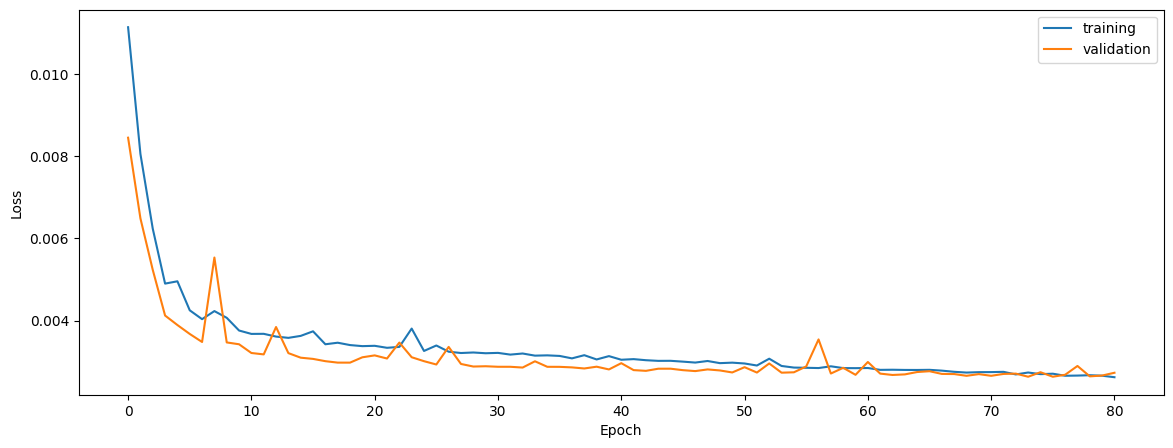
\includegraphics[width=0.7\textwidth]{fa_curve}
\caption{Training Curve: Diffusion Fractional Anisotropy}
\label{fig:curve-fa}
\end{figure}

\begin{figure}[H]
\centering
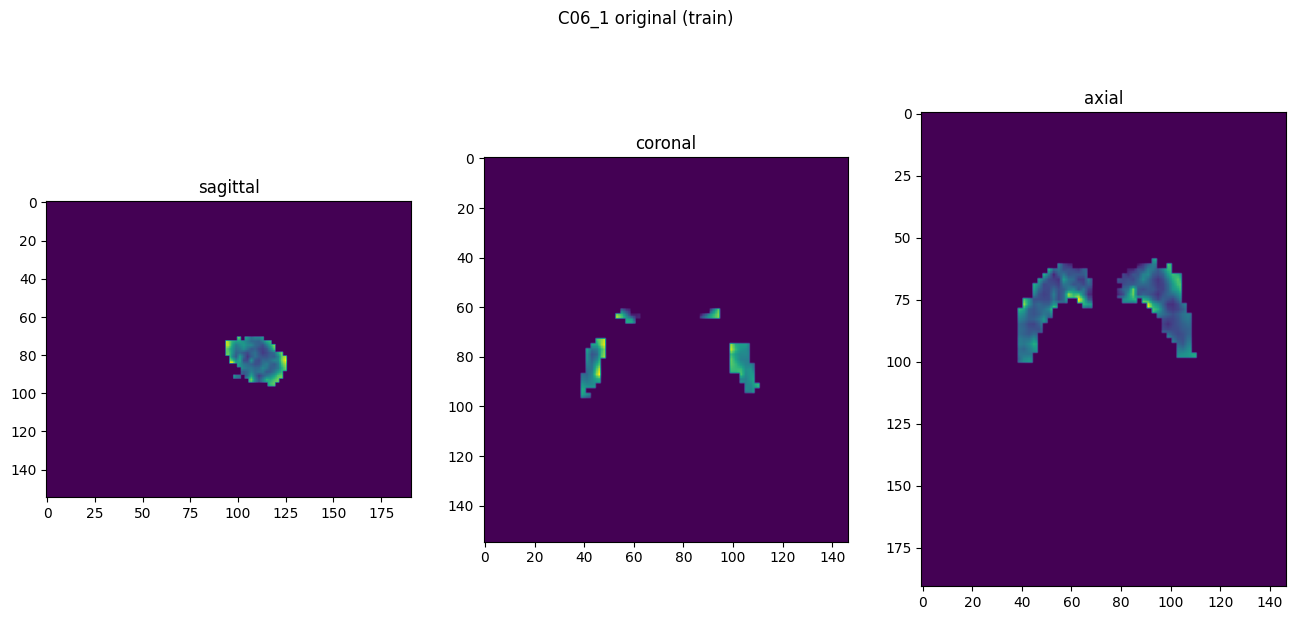
\includegraphics[width=0.65\textwidth]{fa_train_o}
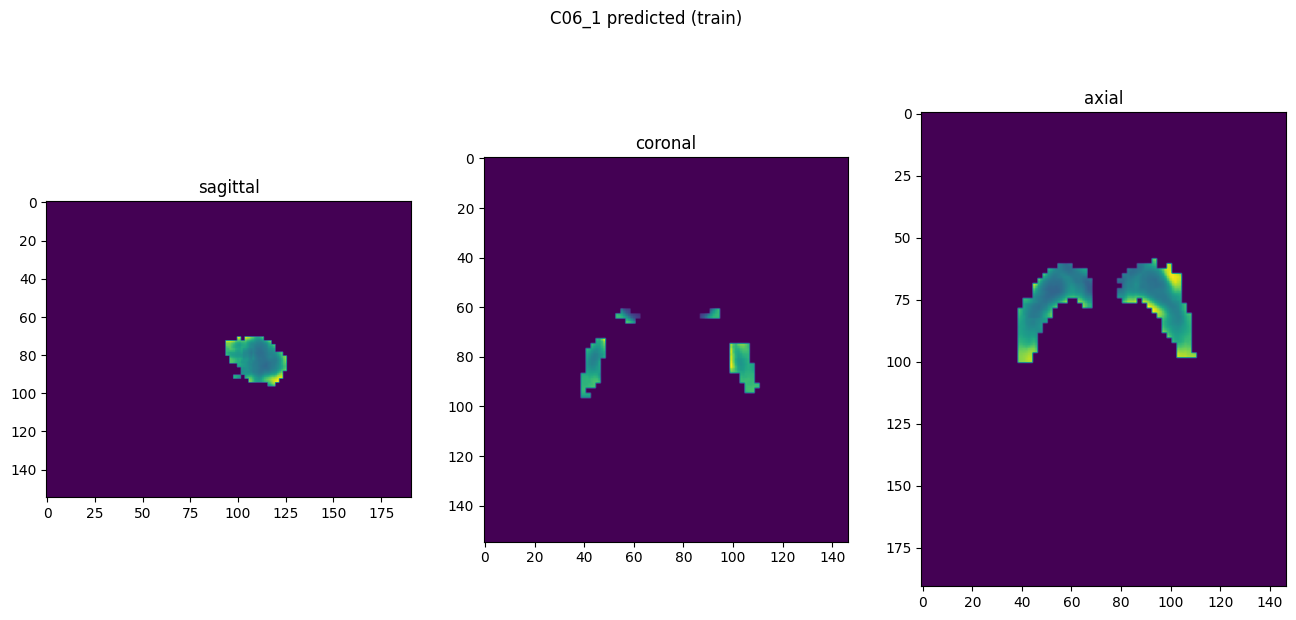
\includegraphics[width=0.65\textwidth]{fa_train_p}
\caption{Train Predictions: Diffusion Fractional Anisotropy}
\label{fig:pred-tra-fa}
\end{figure}

\begin{figure}[H]
\centering
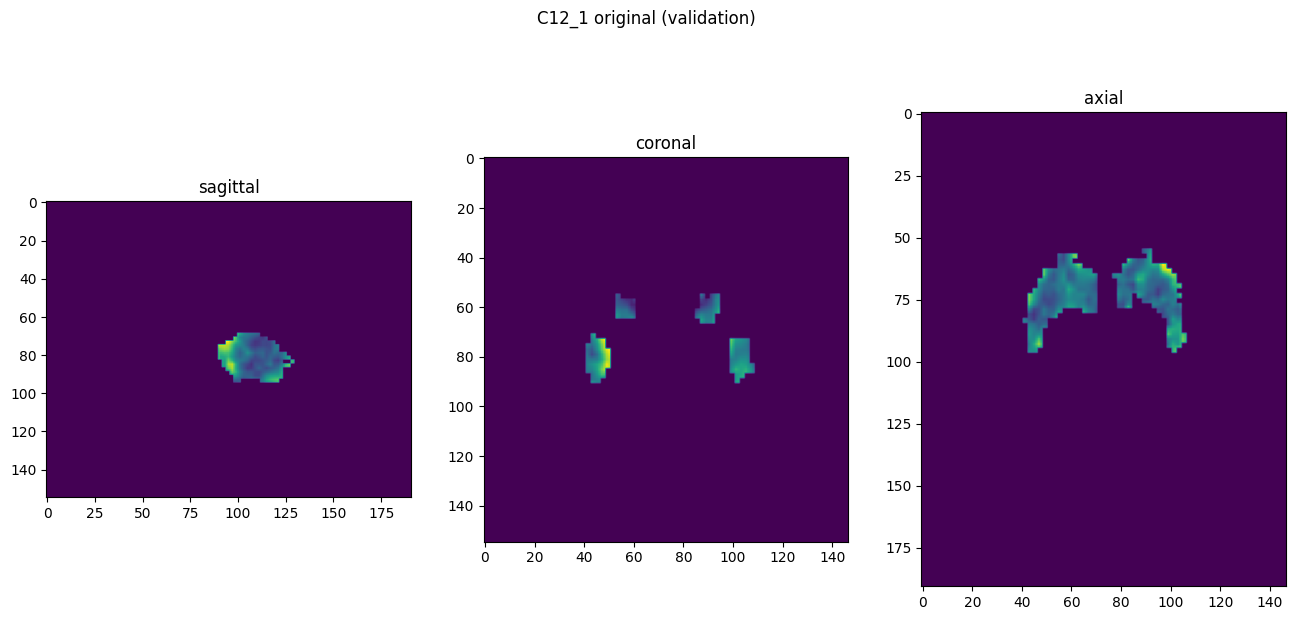
\includegraphics[width=0.65\textwidth]{fa_val_o}
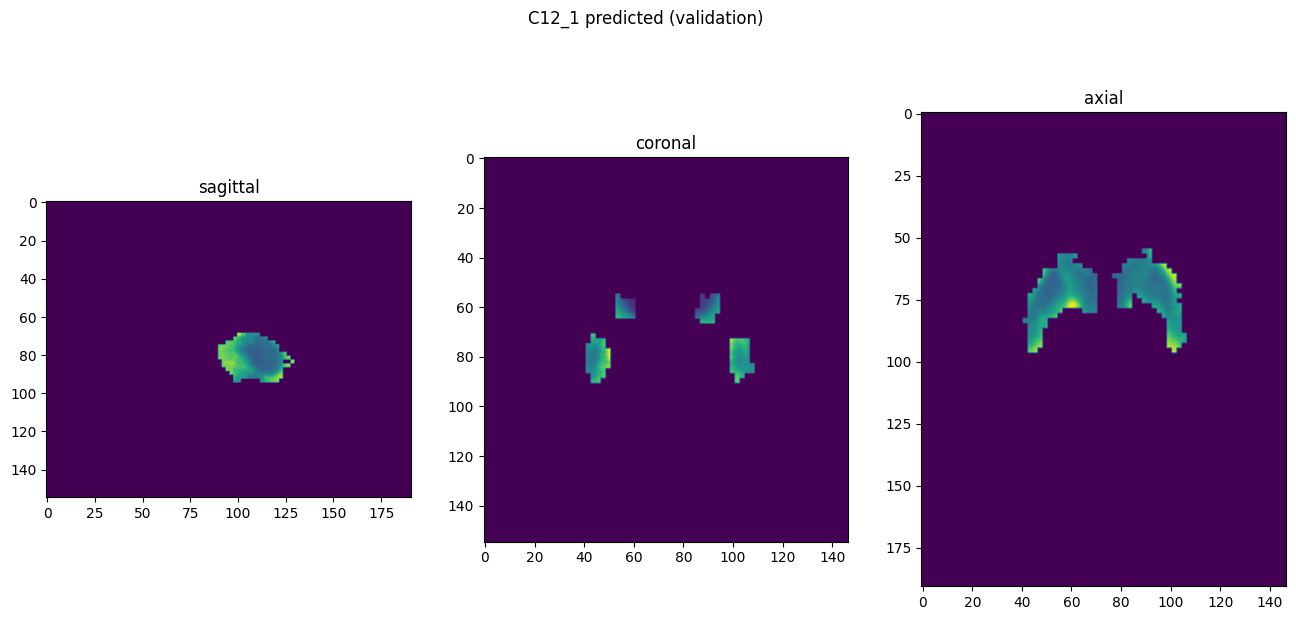
\includegraphics[width=0.65\textwidth]{fa_val_p}
\caption{Validation Predictions: Diffusion Fractional Anisotropy}
\label{fig:pred-val-fa}
\end{figure}

\begin{figure}[H]
\centering
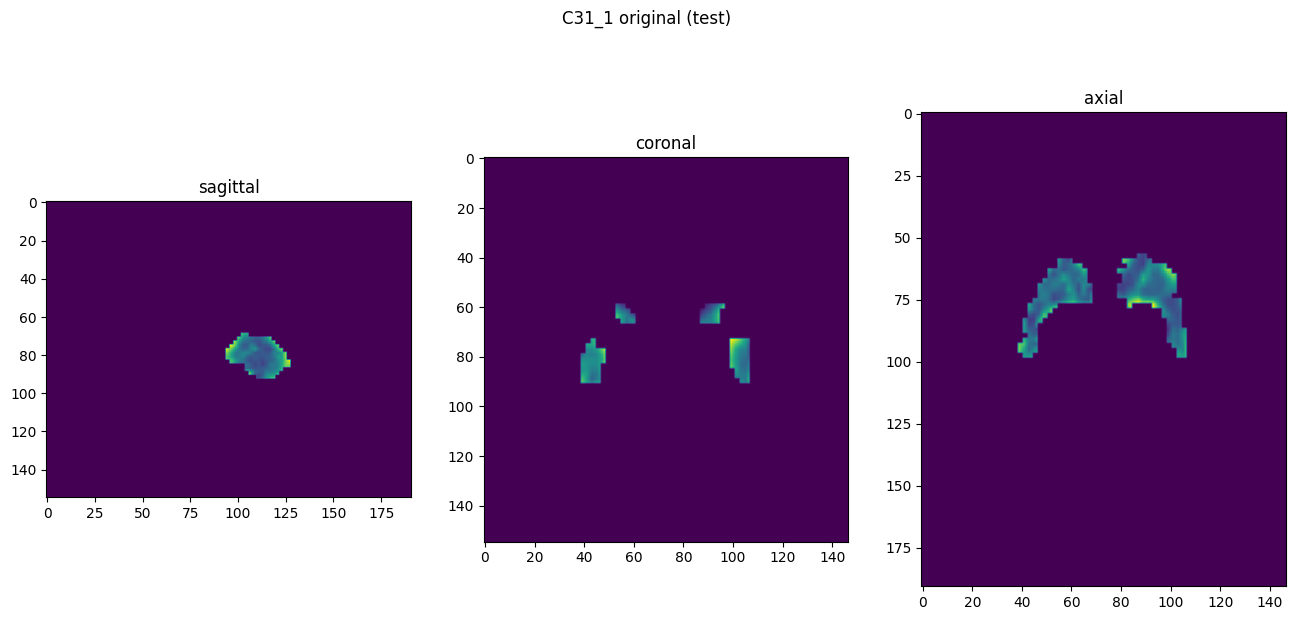
\includegraphics[width=0.65\textwidth]{fa_test_o}
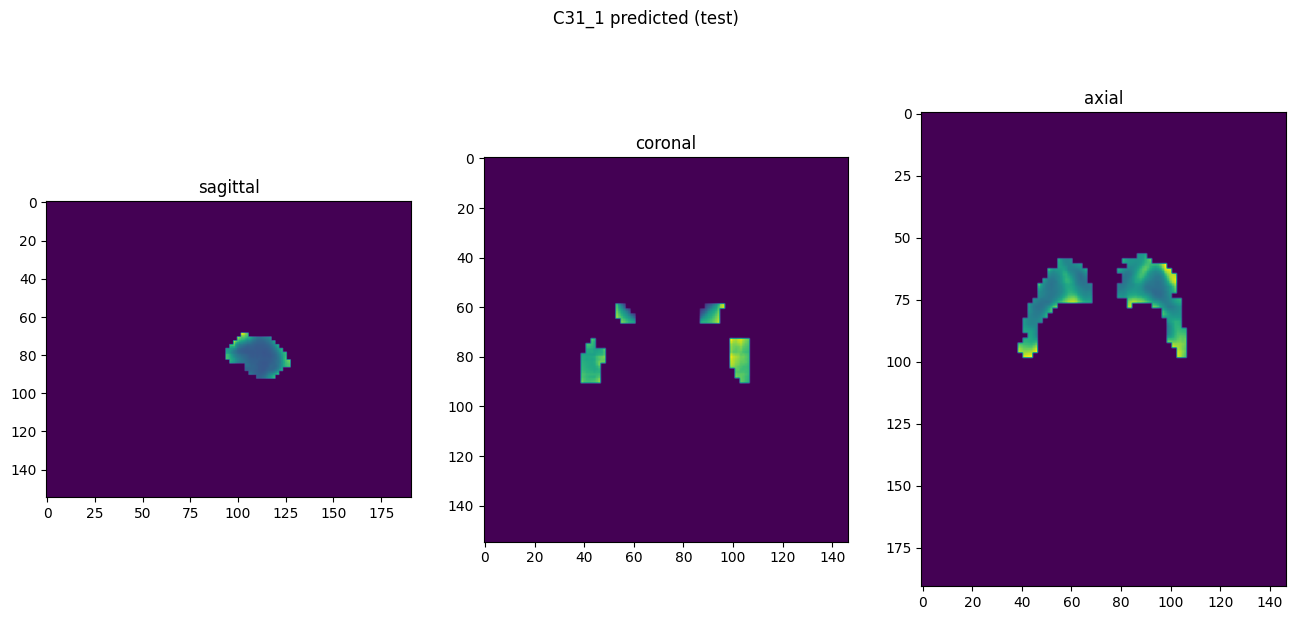
\includegraphics[width=0.65\textwidth]{fa_test_p}
\caption{Test Predictions: Diffusion Fractional Anisotropy}
\label{fig:pred-tes-fa}
\end{figure}

\section{Mean Diffusivity Regression}

A similar set of experiments were run for predicting \ac{MD} with the numerical results available in \reflink{fig:md-nat-t1}{Tables} \reflink{fig:md-arch}{-}. But these experiments were performing very well out of the box, even the baseline Native T1 experiment with a single set of voxel based features resulted in a  correlation of 94\% without any overfitting.\par
No significant observation can be made here, besides the Patient records performing marginally worse.\par
The best performing model was Native T1, on the Control records only, with the additional non-voxel based features of the entire brain, and many different voxel based kernel sizes. It reached a final correlation of \textbf{94.7/95.5/95.1} for the train/val/test splits in native space, and \textbf{95.4/95.7/96.3} in normalized space.\par
After tuning the model architecture, by searching different layer sizes and numbers, activation functions, dropout normalization, adjusting learning rate and batch size, it could not increase the model performance, not even on the train split. Indicating that this is the absolute best this model can do.

\begin{figure}[H]
\centering
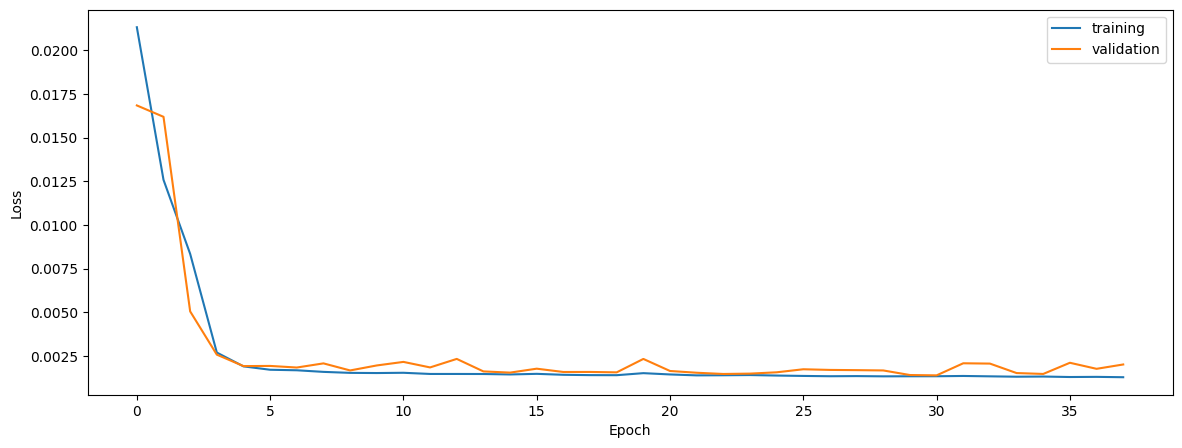
\includegraphics[width=0.7\textwidth]{md_curve}
\caption{Training Curve: Mean Diffusivity}
\label{fig:curve-md}
\end{figure}

\begin{figure}[H]
\centering
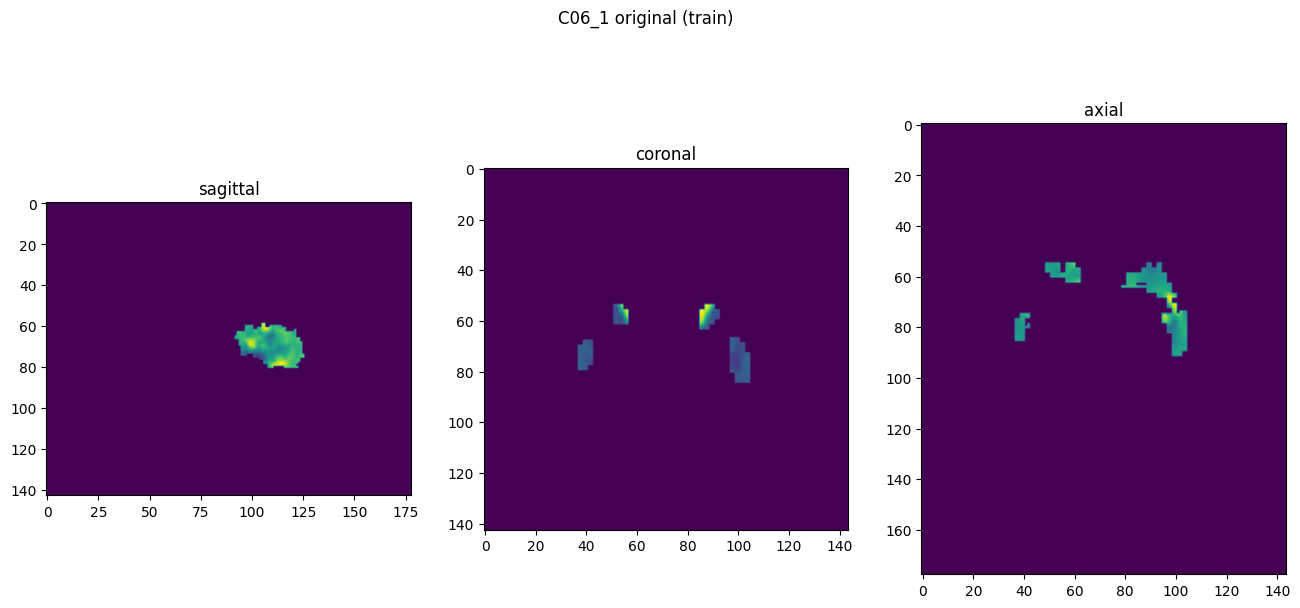
\includegraphics[width=0.65\textwidth]{md_train_o}
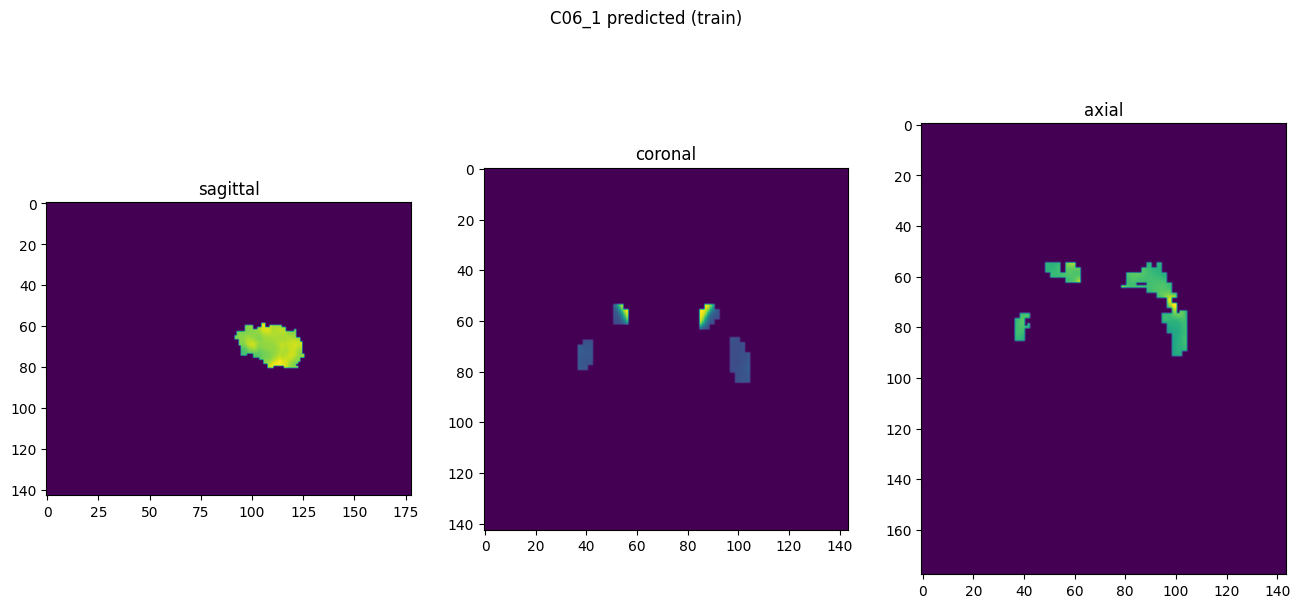
\includegraphics[width=0.65\textwidth]{md_train_p}
\caption{Train Predictions: Mean Diffusivity}
\label{fig:pred-tra-md}
\end{figure}

\begin{figure}[H]
\centering
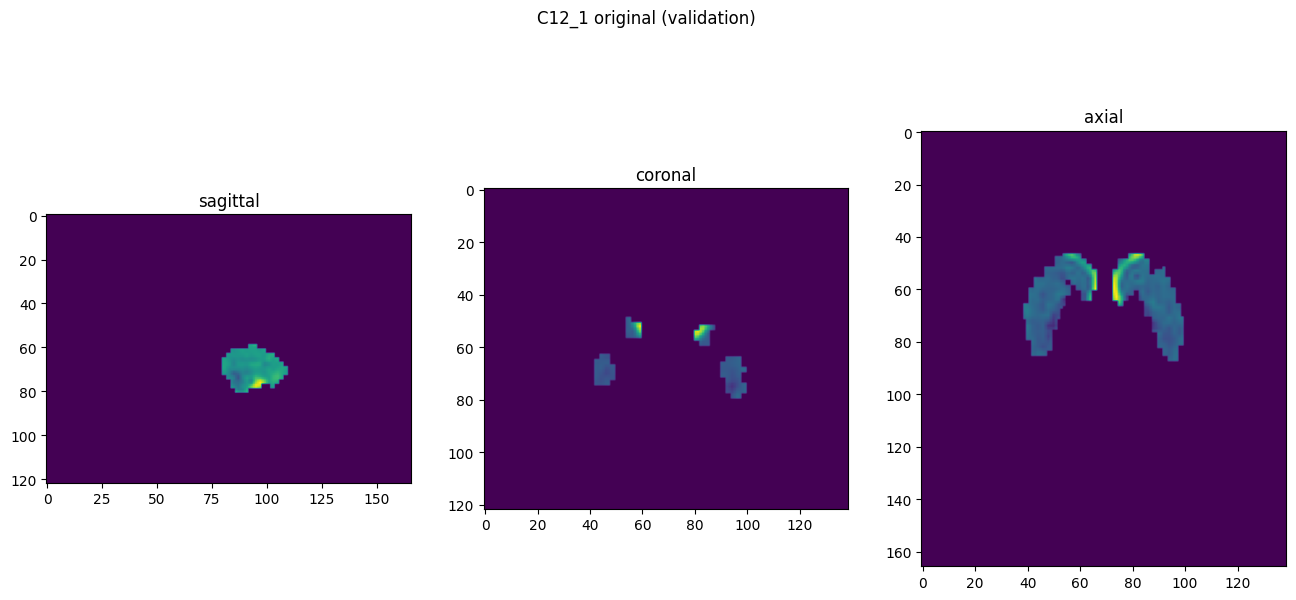
\includegraphics[width=0.65\textwidth]{md_val_o}
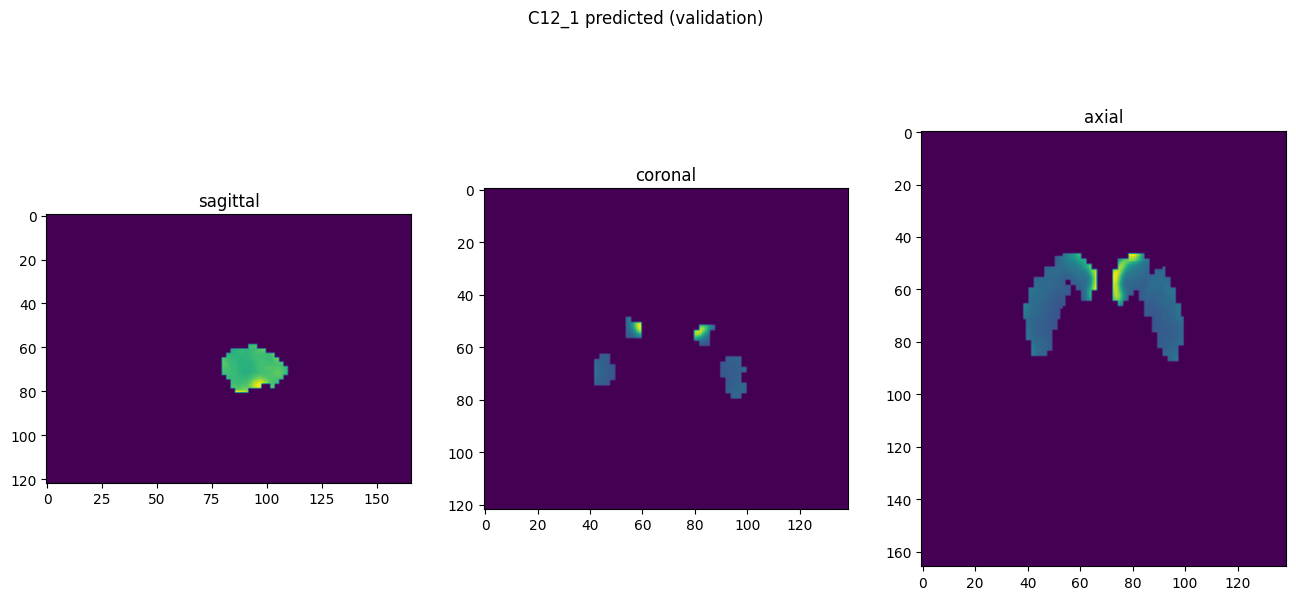
\includegraphics[width=0.65\textwidth]{md_val_p}
\caption{Validation Predictions: Mean Diffusivity}
\label{fig:pred-val-md}
\end{figure}

\begin{figure}[H]
\centering
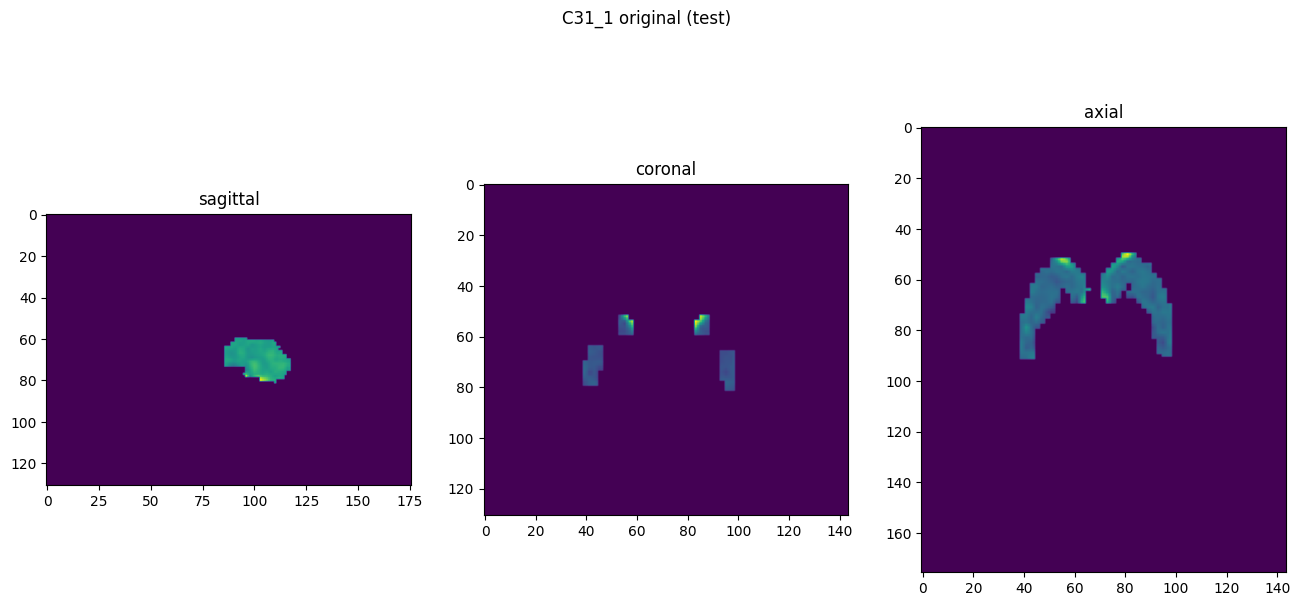
\includegraphics[width=0.65\textwidth]{md_test_o}
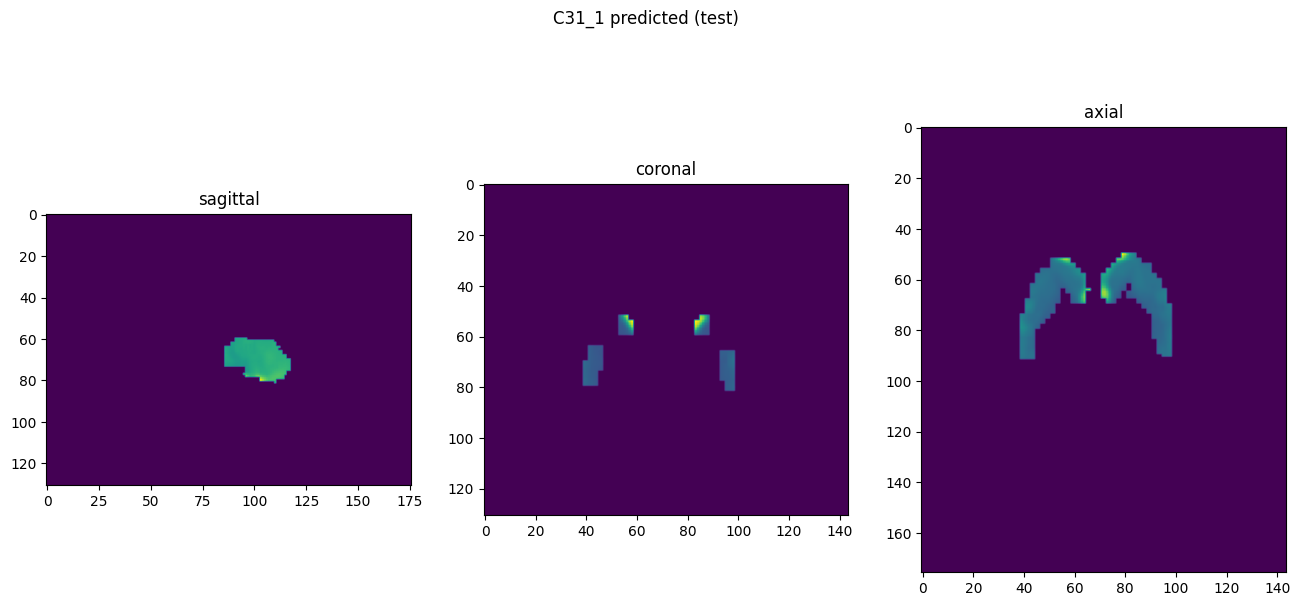
\includegraphics[width=0.65\textwidth]{md_test_p}
\caption{Test Predictions: Mean Diffusivity}
\label{fig:pred-tes-md}
\end{figure}

\section{Relative Connectivity Segmentation}

All numerical results of the experiments can be found in \reflink{fig:con-nat-t1}{Tables} \reflink{fig:con-arch}{-}.
The baseline starting experiment is trying to predict the Relative Connectivity (preprocessed with the method described in \reflink{sec:conpre}{subsection}) from a single set of voxel based radiomic features, with a kernel size of 5. And with the same starting hyperparameters (\reflink{tab:subhyp}{Table}) that were also used in the subcortical segmentation.\par
The next few experiments were trying to determine how does each set (target regions, roi, and entire brain) of non-voxel based features affect the model performance. Between the 4 different group of experiments (Native-Normalized \& T1-T1/T2) the observations were more or less consistent, with the final consensus being that the inclusion of non-voxel based features does not increase model performance.\par
The biggest improvement was the inclusion of many different kernel sized voxel-based features, with an improvement of 5-10\%.\par
The experiments consistently showed the model performing much better on the Control records, compared to the Patient records, with much less overfitting and better accuracy by 2-5\%.\par
The inclusion of the clinical features were behaving inconsistently between the 4 groups of experiments. For the normalized experiments, it mostly had no effect, or made it marginally worse. And for the native T1 experiments, including \ac{CAP} and \ac{cUHDRS} features marginally improved the model performance. And for the native T1/T2 it increased train/validation performance subtantially, but yielded worse test performance, overfitting a lot.\par
Mixing Control and Patient records only performed marginally worse than using only Control records.\par
Including coordinates, consistently increased accuracy by 1-2\%.\par
Only using min-max scaling, and not normalizing the datapoints, resulted in marginally worse performance.\par
Increasing the bin size for the voxel based radiomic features marginally decreased the model performance.\par
Balancing the data consistently decreased performance by quite a lot, depending on the balance ratio by 5-20\%.\par
Re-including the 10 extra T1 records as part of the training split for the T1 experiments did not affect the model performance.\par
After combining all of the best configurations, the best performing model was the T1 normalized model, with Control records only, with the additional coordinate inputs, without any additional non-voxel based features. It reached a final accuracy of 72.6/72.1/73.3 for the train/val/test splits in native space, and 73.2/71.9/73 in normalized space.\par
After tuning the model architecture, by searching different layer sizes and numbers, activation functions, dropout normalization, adjusting learning rate and batch size, the only thing which marginally increased model performance was lowering the batch size to $10^3$ and lowering the learning rate to $10^{-4}$, yielding a final accuracy of \textbf{73.3/72.9/73.4} in native space, and \textbf{73.5/72.3/73.4} in normalized space.\par
As these numbers can be misleading due to the highly unbalanced data, and the best way to get more insight on how the model is performing, is by observing the confusion matrices in \reflink{fig:conf_prec}{Figure} and \reflink{fig:conf_rec}{Figure}. Where matrices in the prior \reflink{fig:conf_prec}{Figure} are normalized along the predicted label axis, effectively displaying the precision on the diagonals; and in the latter \reflink{fig:conf_rec}{Figure} are normalized along the true label axis, effectively displaying the recall on the diagonals. The first and most evident observation is that the unbalanced nature of the data is reflected on the confusion matrix, as the over represented 'not connected' datapoints have a much better precision and recall than the rest.\par
Also, the model is more effective at minimizing false positives, than false negatives, since it generally has a higher precision than recall for practically all labels (except the 'not connected').

\begin{figure}[H]
\centering
\begin{subfigure}{0.49\textwidth}
  \centering
  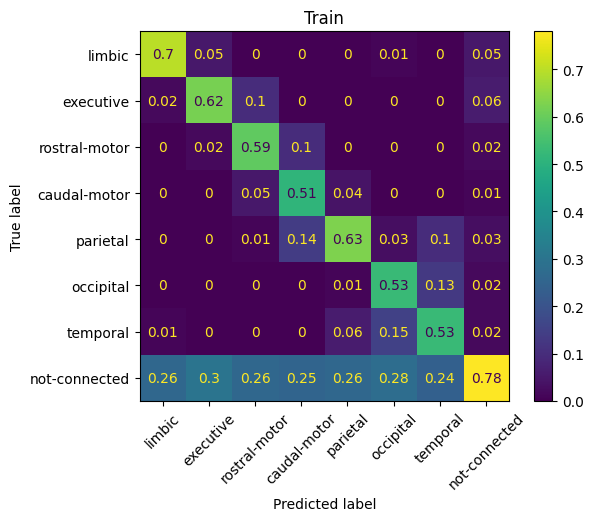
\includegraphics[width=\textwidth]{con_mat_prec_train}
\end{subfigure}
\hfill
\begin{subfigure}{0.49\textwidth}
  \centering
  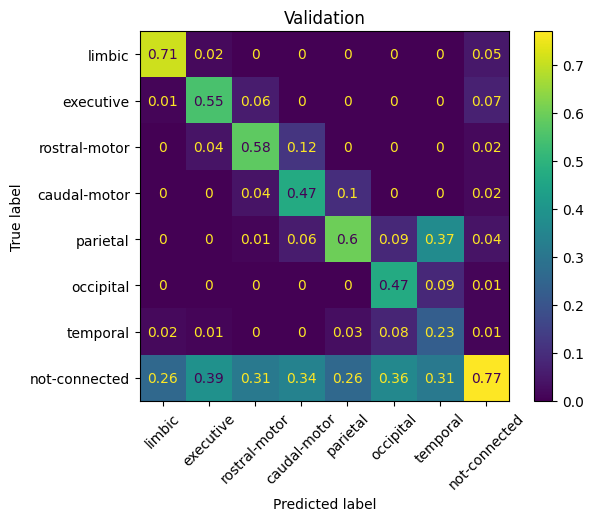
\includegraphics[width=\textwidth]{con_mat_prec_val}
\end{subfigure}
\begin{subfigure}{0.49\textwidth}
  \centering
  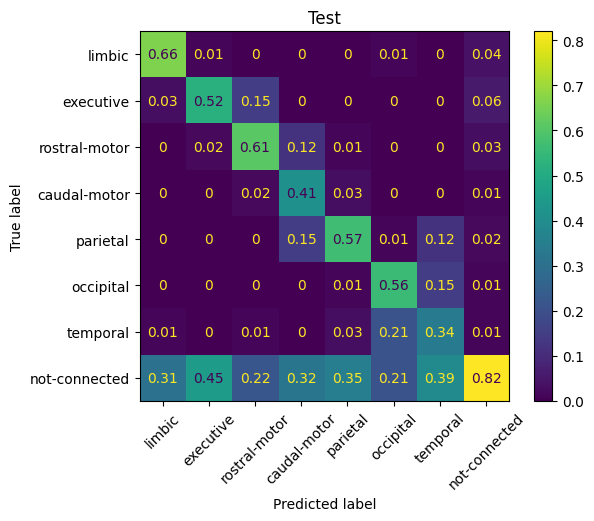
\includegraphics[width=\textwidth]{con_mat_prec_test}
\end{subfigure}
\caption{Confusion Matrices (Precision): Relative Connectivity}
\label{fig:conf_prec}
\end{figure}

These matrices also tell that not all labels are performing equally. As the model clearly struggles with the recall of 'temporal' target region datapoints.

\begin{figure}[H]
\centering
\begin{subfigure}{0.49\textwidth}
  \centering
  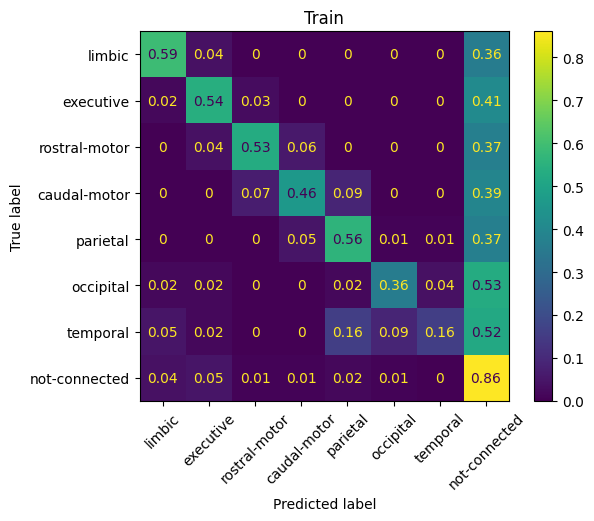
\includegraphics[width=\textwidth]{con_mat_rec_train}
\end{subfigure}
\hfill
\begin{subfigure}{0.49\textwidth}
  \centering
  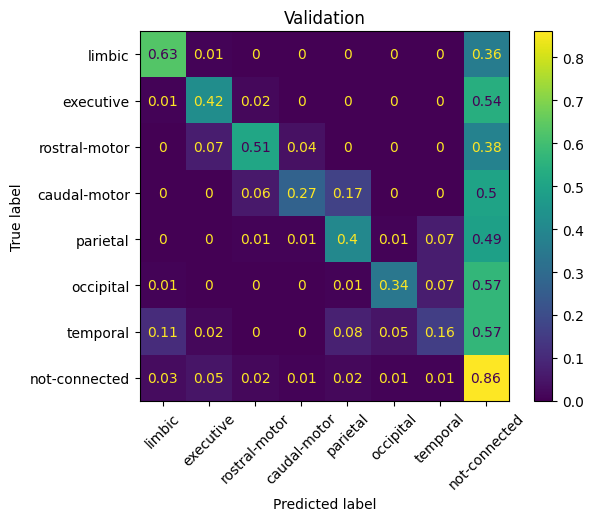
\includegraphics[width=\textwidth]{con_mat_rec_val}
\end{subfigure}
\begin{subfigure}{0.49\textwidth}
  \centering
  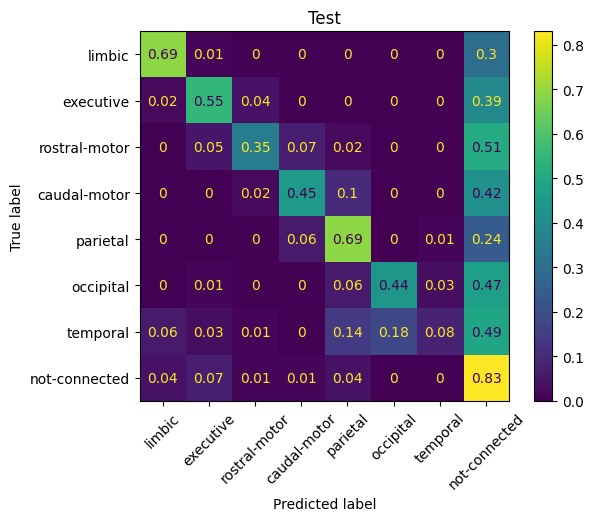
\includegraphics[width=\textwidth]{con_mat_rec_test}
\end{subfigure}
\caption{Confusion Matrices (Recall): Relative Connectivity}
\label{fig:conf_rec}
\end{figure}

\begin{figure}[H]
\centering
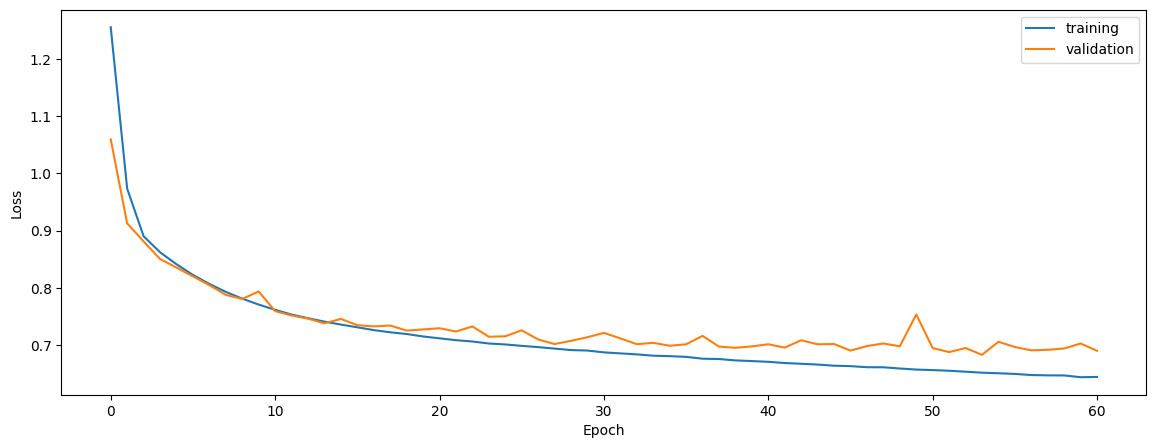
\includegraphics[width=0.7\textwidth]{con_curve}
\caption{Training Curve: Relative Connectivity}
\label{fig:curve-con}
\end{figure}

\begin{figure}[H]
\centering
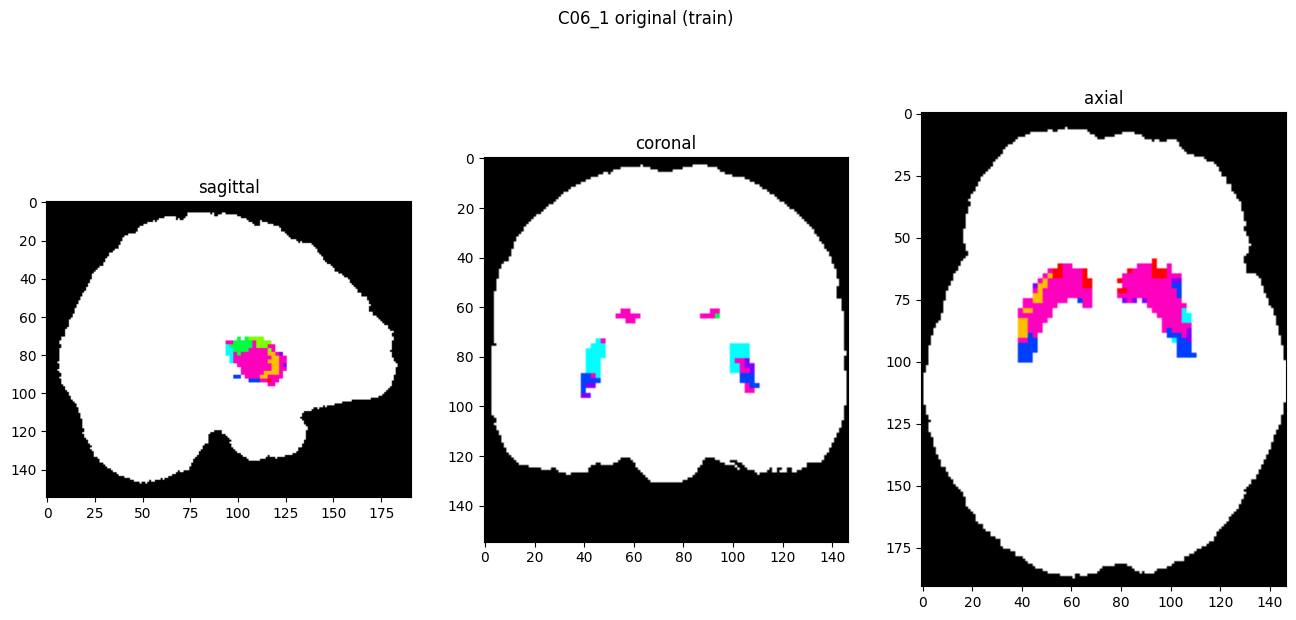
\includegraphics[width=0.65\textwidth]{con_train_o}
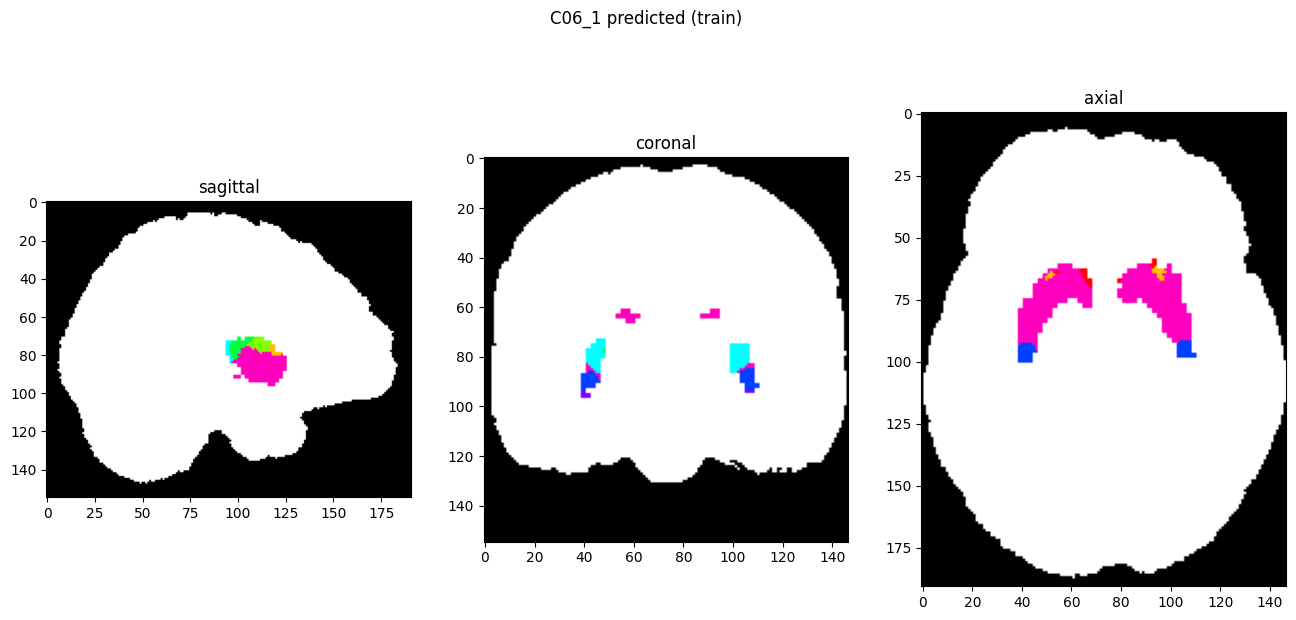
\includegraphics[width=0.65\textwidth]{con_train_p}
\caption{Train Predictions: Relative Connectivity}
\label{fig:pred-tra-con}
\end{figure}

\begin{figure}[H]
\centering
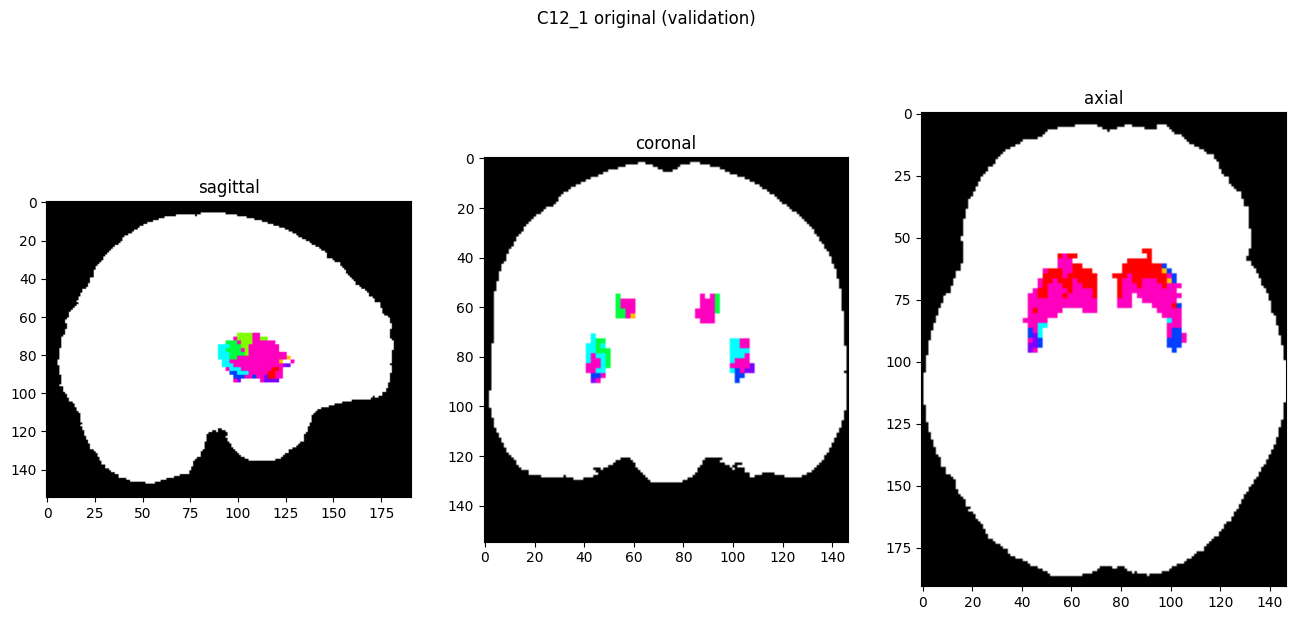
\includegraphics[width=0.65\textwidth]{con_val_o}
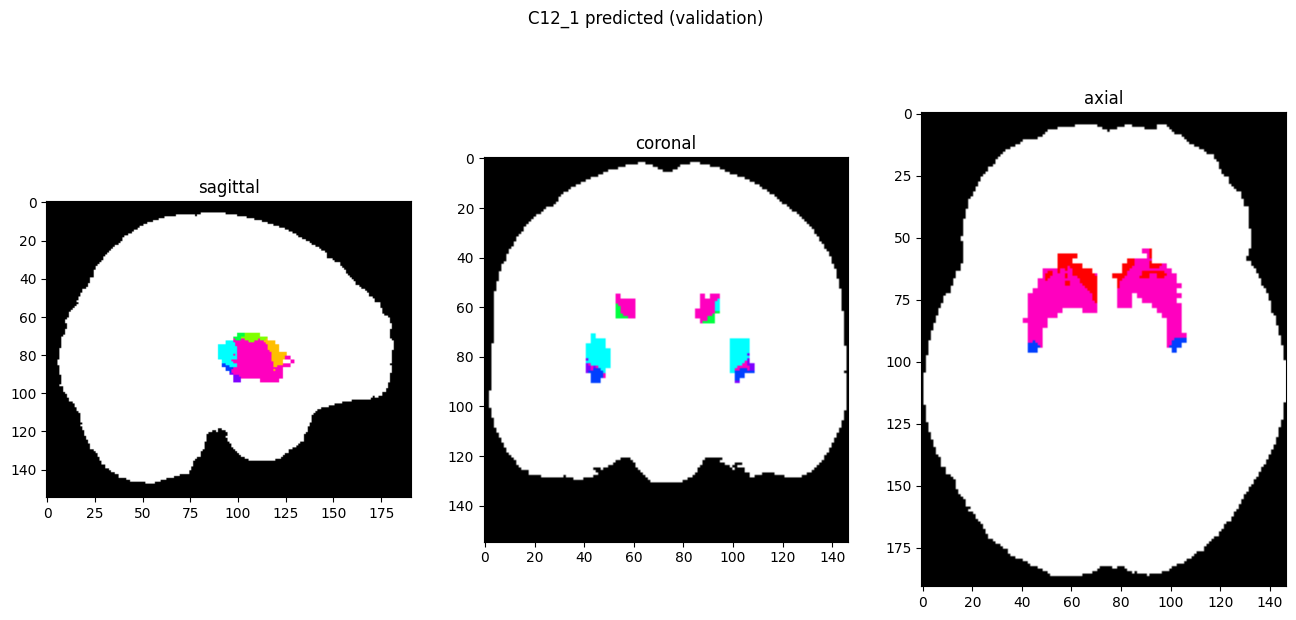
\includegraphics[width=0.65\textwidth]{con_val_p}
\caption{Validation Predictions: Relative Connectivity}
\label{fig:pred-val-con}
\end{figure}

\begin{figure}[H]
\centering
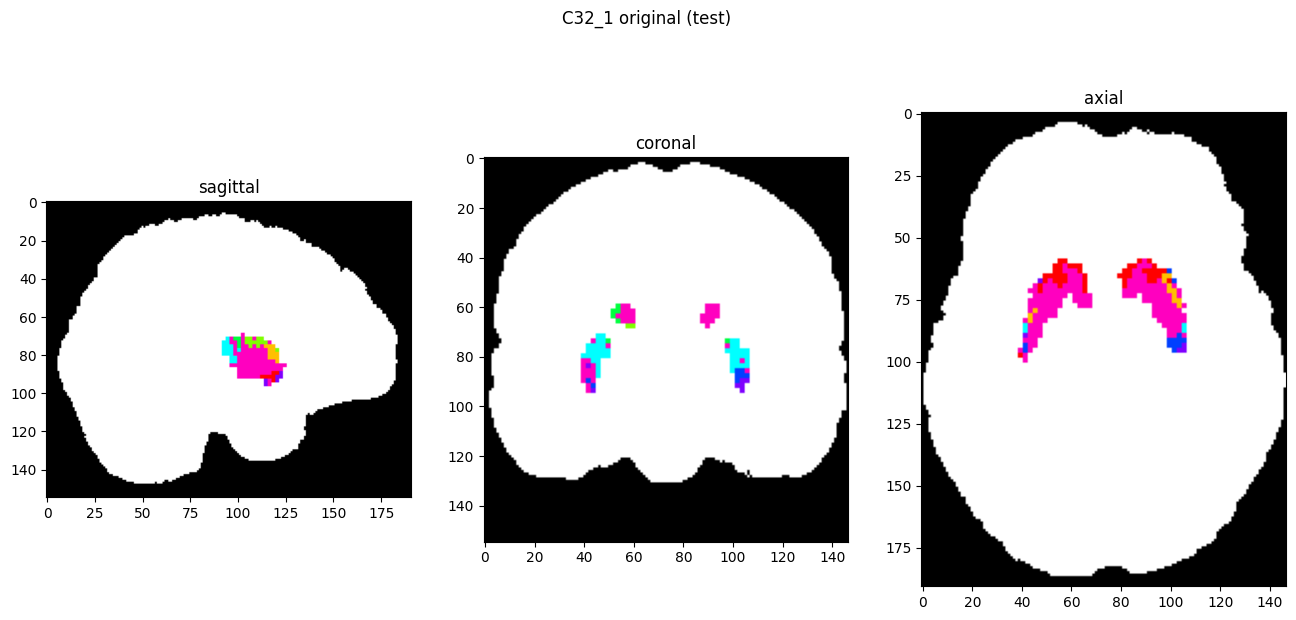
\includegraphics[width=0.65\textwidth]{con_test_o}
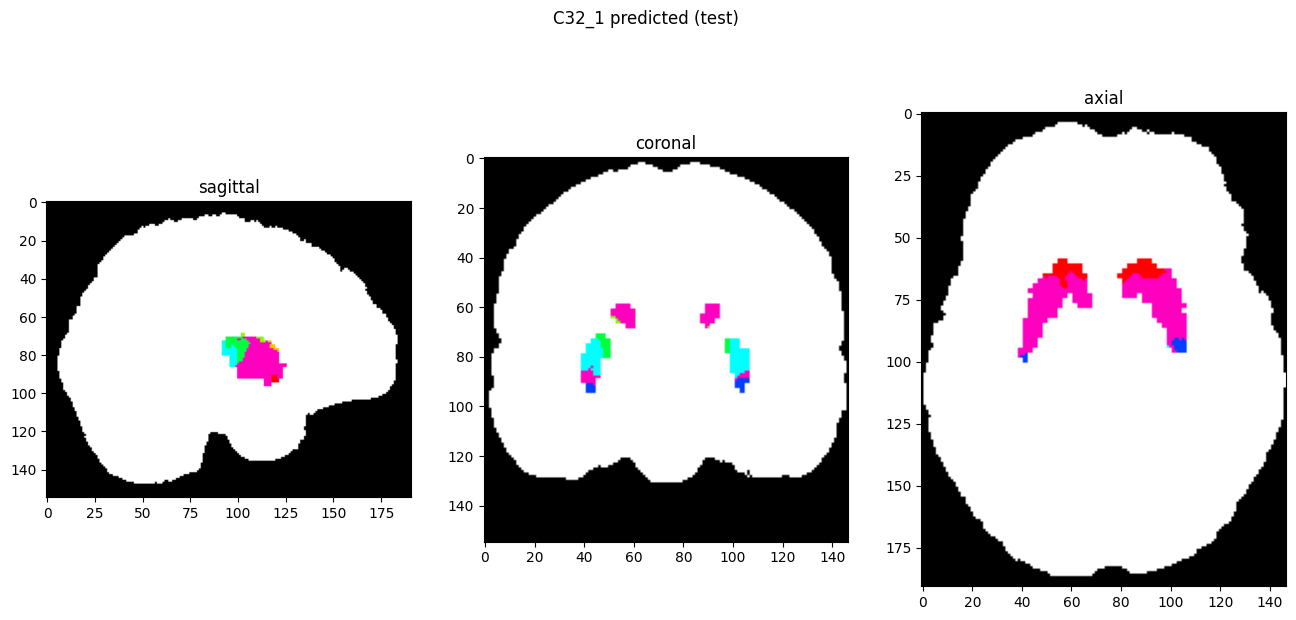
\includegraphics[width=0.65\textwidth]{con_test_p}
\caption{Test Predictions: Relative Connectivity}
\label{fig:pred-tes-con}
\end{figure}

\subsection{Exhaustive Sequential Backwards Feature Selection}
\label{sec:seqback}

Exhaustive sequential backwards feature selection, is a about training the model iteratively by removing a single feature at a time, going through all features. After an iteration is done, the best performing model is chosen, and the corresponding feature is permanently removed before the next iteration, where the model goes through the remaining $n-1$ features.\par
And the stopping criteria can be varied from setup to setup, but in this case the evaluation metric was chosen to be the validation raw accuracy, and a stopping point of where all runs in the iteration performed worse than the baseline (the model with all features included) by more than 2\%.\par
Feature selection was only ran for the Relative Connectivity Segmentation problem, due to it being time consuming and computationally intensive. This was executed on a network cluster, where the cluster head would give out tasks (a task being a model to train with a set of features to exclude), and the workers returning the validation accuracy.\par
There were 2 logistical oversights that were not mitigated in time. The first mistake being that the execution of the feature selection was rushed due to the longevity of the task, and the rest of the hyperparameters (besides the excluded features) were chosen before finishing the basic experimentation. And the second being an indirect consequence to it being rushed, and it was the usage of a bugy code that was responsible for balancing the data, as the bug was found after already executing the feature selection.\par
Due to these mistakes, the selected features turned out not to be very efficient with the final hyperparameters. The feature selection was not executed again due to time and resource limitations. More information detailing this mistake and oversight can be found in \reflink{sec:improve}{Future Improvements} subsection.\par
Nevertheless the expected result of re-running the feature selection would be something similar to the current sub-optimal result. Where around 1/3rd of the features could be excluded before stopping and a maximum increase of 2\% for the validation accuracy. The first features to be excluded was predominantly from the firstorder feature class, followed by the \ac{GLCM} feature class.

\begin{longtable}[H]{|l|l|l|}
\hline
\textbf{Iteration} & \textbf{Excluded Feature} & \textbf{Accuracy} \\ \hline
0. & BASELINE & 59.0 \\ \hline
1. & firstorder\_MeanAbsoluteDeviation & 59.6 \\ \hline
2. & firstorder\_Entropy & 59.9 \\ \hline
3. & firstorder\_Energy & 58.7 \\ \hline
4. & glszm\_SmallAreaLowGrayLevelEmphasis & 58.5 \\ \hline
5. & firstorder\_90Percentile & 59.3 \\ \hline
6. & glcm\_Autocorrelation & 59.5 \\ \hline
7. & firstorder\_Mean & 59.4 \\ \hline
8. & firstorder\_Maximum & 59.1 \\ \hline
9. & glszm\_LowGrayLevelZoneEmphasis & 58.9 \\ \hline
10. & glcm\_Imc1 & 60.0 \\ \hline
11. & firstorder\_Median & 60.1 \\ \hline
12. & glszm\_ZoneVariance & 59.3 \\ \hline
13. & firstorder\_TotalEnergy & 58.9 \\ \hline
14. & firstorder\_10Percentile & 60.4 \\ \hline
15. & firstorder\_Minimum & 59.1 \\ \hline
16. & glszm\_SmallAreaHighGrayLevelEmphasis & 59.9 \\ \hline
17. & firstorder\_InterquartileRange & 60.0 \\ \hline
18. & firstorder\_Kurtosis & 59.6 \\ \hline
19. & firstorder\_RobustMeanAbsoluteDeviation & 59.3 \\ \hline
20. & firstorder\_RootMeanSquared & 59.8 \\ \hline
21. & gldm\_LargeDependenceEmphasis & 58.9 \\ \hline
22. & firstorder\_Variance & 59.1 \\ \hline
23. & glcm\_DifferenceAverage & 59.4 \\ \hline
24. & firstorder\_Uniformity & 58.9 \\ \hline
25. & firstorder\_Skewness & 59.0 \\ \hline
26. & firstorder\_Range & 58.6 \\ \hline
27. & glcm\_JointAverage & 58.7 \\ \hline
28. & glcm\_ClusterProminence & 59.2 \\ \hline
29. & glcm\_ClusterTendency & 58.5 \\ \hline
30. & glcm\_ClusterShade & 60.2 \\ \hline
31. & glcm\_Correlation & 60.0 \\ \hline
32. & glcm\_DifferenceEntropy & 58.1 \\ \hline
33. & glrlm\_RunVariance & 59.3 \\ \hline
34. & glcm\_JointEnergy & 59.6 \\ \hline
35. & glcm\_Contrast & 60.5 \\ \hline
36. & glcm\_Idm & 59.3 \\ \hline
37. & glcm\_Imc2 & 58.7 \\ \hline
38. & glcm\_DifferenceVariance & 59.2 \\ \hline
39. & glcm\_Idmn & 58.0 \\ \hline
40. & glcm\_MCC & 57.9 \\ \hline
41. & glcm\_JointEntropy & 56.6 \\ \hline
\caption{Feature Selection}
\end{longtable}

\subsection{Streamline Regression}

Another approach would be to try predicting the raw streamline images, and then process the predictions the same way as the relative connectivity labels were computed in the first place. This method could result in a more robust solution with predicting a the upstream data, before preprocessing.\par

Training 7 expert models for the 7 streamline images (to each cortical target), with the same hyperparameters as the best performing model from the relative connectivity segmentation, yielded underwhelming results. With the computed accuracies being 65.1/65.3/63.8, and terrible precision/recall on all labels (except the 'not connected'), which is explained by the predicted labels mainly being 'not connected'.\par

This approach was not explored further in depth due to limited time and resources.




